\documentclass[border=3pt]{standalone}
% Preâmbulo compartilhado pelos diagramas TikZ da aula 8 de IHC (Design de IHC)
\usepackage[T1]{fontenc}
\usepackage[utf8]{inputenc}
\usepackage{lmodern}
\usepackage{amsmath}
\usepackage{xcolor}
\usepackage{tikz}
\usetikzlibrary{arrows.meta,angles,quotes,decorations.pathmorphing,decorations.pathreplacing,calc,
                positioning,shapes.geometric,shapes.misc,backgrounds,fit,
                math}

% Paleta (mesma dos SVGs originais)
% Paleta da disciplina de IHC: acento roxo (#755099), da capa do livro.
% (o nome "dblue" é mantido para não alterar todos os diagramas)
\definecolor{dblue}{HTML}{755099}
\definecolor{dorange}{HTML}{B3541E}
\definecolor{dgreen}{HTML}{4A7C59}
\definecolor{dred}{HTML}{9C4B4B}
\definecolor{dcream}{HTML}{F4F1EA}
\definecolor{dshade}{HTML}{DDD7C9}

% Função gaussiana (não normalizada por padrão de escala visual)
\pgfmathdeclarefunction{gauss}{3}{%
  \pgfmathparse{1/(#3*sqrt(2*pi))*exp(-((#1-#2)^2)/(2*#3^2))}%
}

% Estilos comuns (prefixo d... para não colidir com chaves internas do pgf)
\tikzset{
  >={Stealth[length=2mm]},
  dguide/.style={gray!55, dashed, line width=0.4pt},
  daxis/.style={gray!60, line width=0.7pt, ->},
  dbody/.style={fill=black!3, draw=black!80, line width=1pt},
  dacc/.style={draw=dblue, line width=1pt},
  dlbl/.style={black!55, font=\small},
  dsub/.style={black!45, font=\footnotesize},
  dstate/.style={circle, draw=black!80, fill=dcream, line width=1pt,
                 minimum size=17mm, font=\large, inner sep=1pt},
  dobs/.style={circle, draw=black!80, fill=dshade, line width=1pt,
               minimum size=14mm, font=\large, inner sep=1pt},
  dbox/.style={rounded corners=2pt, draw=black!80, fill=dcream, line width=1pt,
               align=center, inner sep=6pt},
  dop/.style={circle, draw=black!80, fill=white, line width=1pt,
              minimum size=6mm, inner sep=0pt, font=\small},
  dtrans/.style={->, dblue, line width=1pt},
  dmeas/.style={->, dorange, line width=1pt},
  dcurve/.style={line width=1pt, dblue},
  dcurveb/.style={line width=1.4pt, dorange},
}

\begin{document}
\hyphenpenalty=10000 \exhyphenpenalty=10000 \tolerance=9999 \emergencystretch=3em
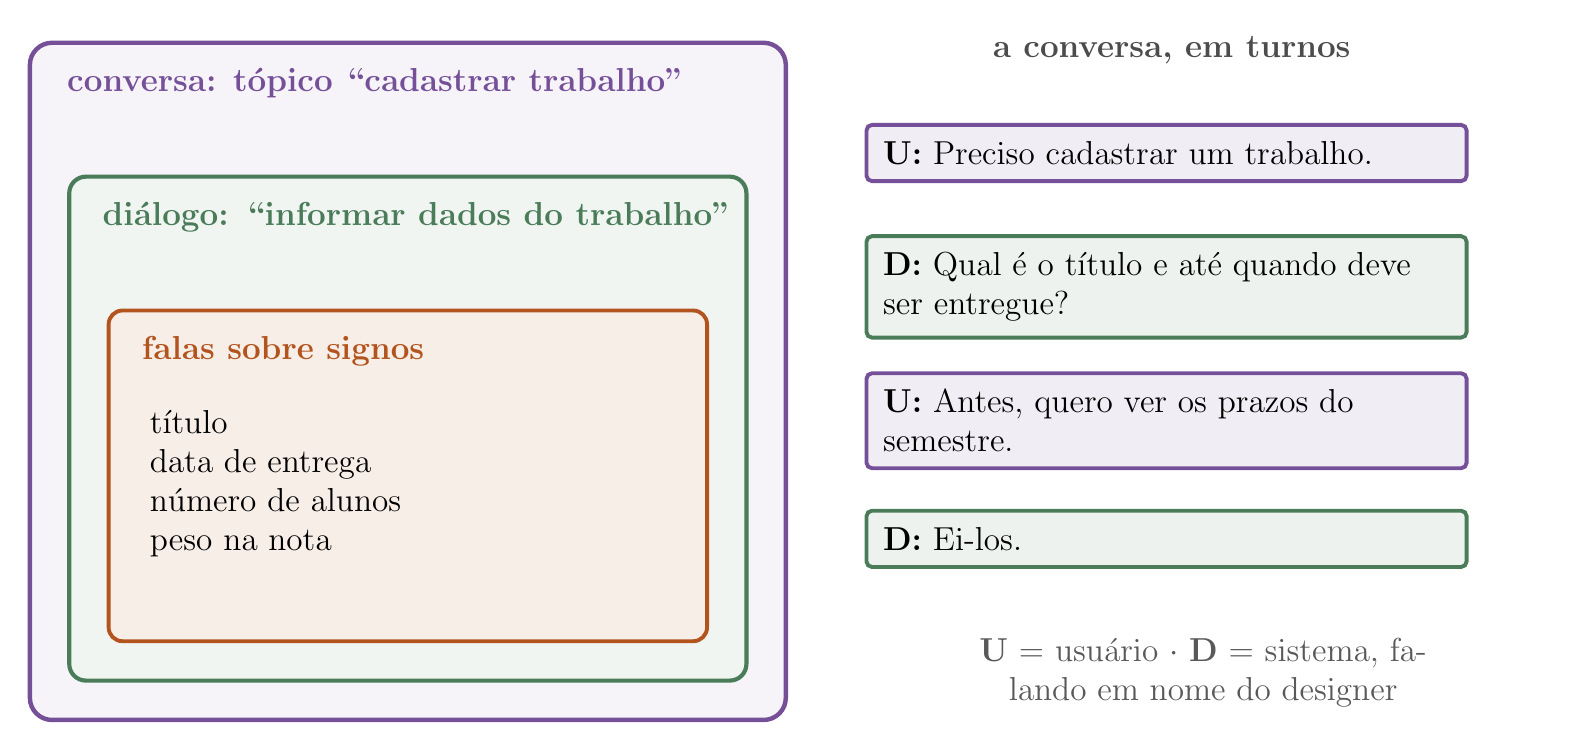
\begin{tikzpicture}[x=1cm,y=1cm]
\draw[dblue, line width=1.6pt, rounded corners=8pt, fill=dblue!6] (0,0) rectangle (9.6,8.6);
\node[font=\large\bfseries, dblue, anchor=north west] at (0.35,8.4) {conversa: tópico ``cadastrar trabalho''};
\draw[dgreen, line width=1.5pt, rounded corners=6pt, fill=dgreen!8] (0.5,0.5) rectangle (9.1,6.9);
\node[font=\large\bfseries, dgreen, anchor=north west] at (0.8,6.7) {diálogo: ``informar dados do trabalho''};
\draw[dorange, line width=1.4pt, rounded corners=5pt, fill=dorange!10] (1.0,1.0) rectangle (8.6,5.2);
\node[font=\large\bfseries, dorange, anchor=north west] at (1.3,5.0) {falas sobre \textbf{signos}};
\node[font=\large, anchor=west, align=left] at (1.4,3.0) {título\\ data de entrega\\ número de alunos\\ peso na nota};
\tikzset{u/.style={dbox, draw=dblue, fill=dblue!10, line width=1.4pt, text width=7.2cm, font=\large, align=left},
        d/.style={dbox, draw=dgreen, fill=dgreen!10, line width=1.4pt, text width=7.2cm, font=\large, align=left}}
\node[font=\large\bfseries, black!70] at (14.5,8.5) {a conversa, em turnos};
\node[u, anchor=west] at (10.6,7.2) {\textbf{U:} Preciso cadastrar um trabalho.};
\node[d, anchor=west] at (10.6,5.5) {\textbf{D:} Qual é o título e até quando deve ser entregue?};
\node[u, anchor=west] at (10.6,3.8) {\textbf{U:} Antes, quero ver os prazos do semestre.};
\node[d, anchor=west] at (10.6,2.3) {\textbf{D:} Ei-los.};
\node[font=\large, black!65, text width=8.4cm, align=center] at (14.9,0.6) {\textbf{U} = usuário $\cdot$ \textbf{D} = sistema, falando em nome do designer};
\end{tikzpicture}
\end{document}
